\documentclass[12p]{article}
\usepackage[utf8]{inputenc}
\usepackage[english]{babel}

\usepackage{graphicx}
\usepackage{hyperref}
\usepackage{caption}
\usepackage{mathtools}
\usepackage{lscape}

\usepackage[backend=biber,style=iso-numeric,sorting=none]{biblatex}
\bibliography{references.bib}

\title{Exoplanet Ranking \\\large Introduction to Data Science}
\date{\today}
\author{Goron, Nathan\and Motzkus, Franz\and Vopat, Tomas
}

%------------------------------------------------------------------
%------------------------------------------------------------------

\begin{document}

\maketitle

\section{Introduction}

In our project we computed a ranking of the already discovered exoplanets in the pursuit of giving first sights of planets that could fit the role of next home for mankind.
Once the ranking is created, we would display it on a website, along with visualisations regarding the dataset.

We think that our study might interest companies, that want to raise people's curiosity around the topic of finding Earth-like planets, or simply astronomy enthusiast, that we can inspire with a new view.

The results of our work take form in two materials; the ranking dataset which features every exoplanet from the original dataset and, associated to each of them, a grade from 0 to 10 representing how suitable they would be as earth replacement.

%------------------------------------------------------------------

\section{Preprocessing and Analysis}
The dataset~\cite{dataset} we used is from an archive hosted by the NASA exoplanet science institute which is operated by the California Institute of Technology. The dataset features 4056 exoplanets.

The data collection includes data from 47 attributes, that contain administrative information like the name of the planet or the planetary system, but also information about metal sources or the luminosity, which can be used for our ranking, since they influence, if humanity could survive on this planet.

As a first step we removed the columns, that seemed to contain data, that is irrelevant for our task (e.g. multiple columns contain links to studies proving the veracity of the data in other columns; since the data is published by an official institute, that works in close relation to the NASA, we rely on the credibility of the data). 

We also dropped columns where a significant amount of data was missing. About a dozen columns of the original 47 columns from the dataset had a missing data ratio of above 75 percent, so interpolating the existing data in these columns would lead to highly distorted results.

Since it needs domain knowledge of physicists, astrologists and maybe even biologists, that we could not provide at this moment, we included most of the attributes into our ranking, that seemed to have a reasonable impact, when computing the similarity of the exoplanet to the Earth. We therefore combined the attribute descriptions in the dataset in combination with easily accessible information from Wikipedia.

In total we reduced the number of attributes to 22 fully-filled and relevant columns for the computation of our ranking. We also added the Earth and it's information to the dataset, as it will be valuable for computing the ranking and visualisations later on. Description of all attributes can be found in Table~\ref{tab:att_desc}.

%------------------------------------------------------------------

\section{Ranking}
The ranking is computed by evaluating the similarity of each exoplanet to the specs of planet Earth based on a the parameters we extracted beforehand such as the surface temperature of the planet, it’s gravity, it’s light exposition, etc. We believe that some parameters probably have a bigger impact than others on how ``livable`` an exoplanet is. For instance, the year of discovery of the planet is probably not as important as it's surface temperature or it's gravitational force. Therefore two rankings have been computed: There is one ranking that doesn't take into account the weight of the parameters, and one that does.

In the so-called weighted ranking, parameters will see themselves attributed a weight coefficient that goes from 0 to 10 , which influences the computed score and therefor results in a different rating. The importance factors that were associated with the attributes were introduced by our sense of understanding on what is important.

The Ranking is computed using the native python-embedded cosine similarity formula, where $u$ and $v$ are the vectors for on exoplanet data row, and $w$ the weight coefficient of a parameter.

\begin{align}
\text{cosine}(u,v) &= \frac{\sum_{i=0}^{n-1} u_iv_i  }{ \sqrt{\sum_{i=0}^{n-1} u_i^2  } \sqrt{\sum_{i=0}^{n-1} v_i^2  }} \label{eq:cosine}\\
\text{cosine}_{\text{weighted}}(u,v,w) &= \frac{\sum_{i=0}^{n-1} (u_i-\overline{u_w})(v_i-\overline{v_w})  }{ \sqrt{\sum_{i=0}^{n-1} (u_i-\overline{u_w})^2  } \sqrt{\sum_{i=0}^{n-1} (v_i-\overline{v_w})^2  }} \label{eq:cosine_weighted} \\
\overline{u_w} &= \frac{ \sum_{i=0}^{n-1} u_iw_i }{ \sum_{i=0}^{n-1} w_i } \label{eq:weighted_mean}
\end{align}

%------------------------------------------------------------------

\section{Webapp}
We then came up with a node.js web application to display the results of our ranking, This website uses native HTML/CSS/JS, a node.js templating engine to pass data to views as well as some data visualisation framework such as chart.js to make it easier to display our data.

The Webapp displays the ten first planets for both the weighted and unweighted ranking.

%------------------------------------------------------------------

\section{Results}
bla, bla,...

%------------------------------------------------------------------

\printbibliography

\appendix

\begin{landscape}
    \section{Dataset Attributes}
    \begin{table}[!h]\centering
        \caption{Attributes Description}
        \label{tab:att_desc}
        \begin{tabular}{|l l c|}\hline
            Attribute         & Description & Weight \\ \hline\hline
            fpl\_orbper      & orbital period (days) & 5 \\ \hline
            fpl\_smax        & the longest radius of an elliptic orbit & 3 \\ \hline
            fpl\_bmasse    & mass of the planet (earth unit) & 5 \\ \hline
            fpl\_rade         & radius (earth unit) & 5 \\ \hline
            fpl\_dens        & density of the planet (g/cm**3) & 7 \\ \hline
            fpl\_tranflag    & wether the lanet transits the star or not & 1 \\ \hline
            fpl\_cbflag      & does planet orbit a binary solar system & 5 \\ \hline
            fpl\_snum       & number of stars in the solar system & 8 \\ \hline
            dec                 & declination of the planetary system & 3 \\ \hline
            fst\_teff          & effective temperature in Kelvins & 10 \\ \hline
            fst\_logg        & gravity acceleration at the star surface log10(cm/s**2) & 4 \\ \hline
            fst\_lum         & star lumonisty log10(lumonisity) & 4 \\ \hline
            fst\_mass       & stellar mass (sun unit) & 6 \\ \hline
            fst\_rad         & stellar raidus (sun unit) & 6 \\ \hline
            fst\_met        & star metallicity & 3 \\ \hline
            fst\_metratio & metal abundance (in comparison to sun) & 1 \\ \hline
            fst\_age         & stellar age (in billions) & 8 \\ \hline
        \end{tabular}
    \end{table}
\end{landscape}

\section{Charts}

\begin{figure}[!ht]\centering
    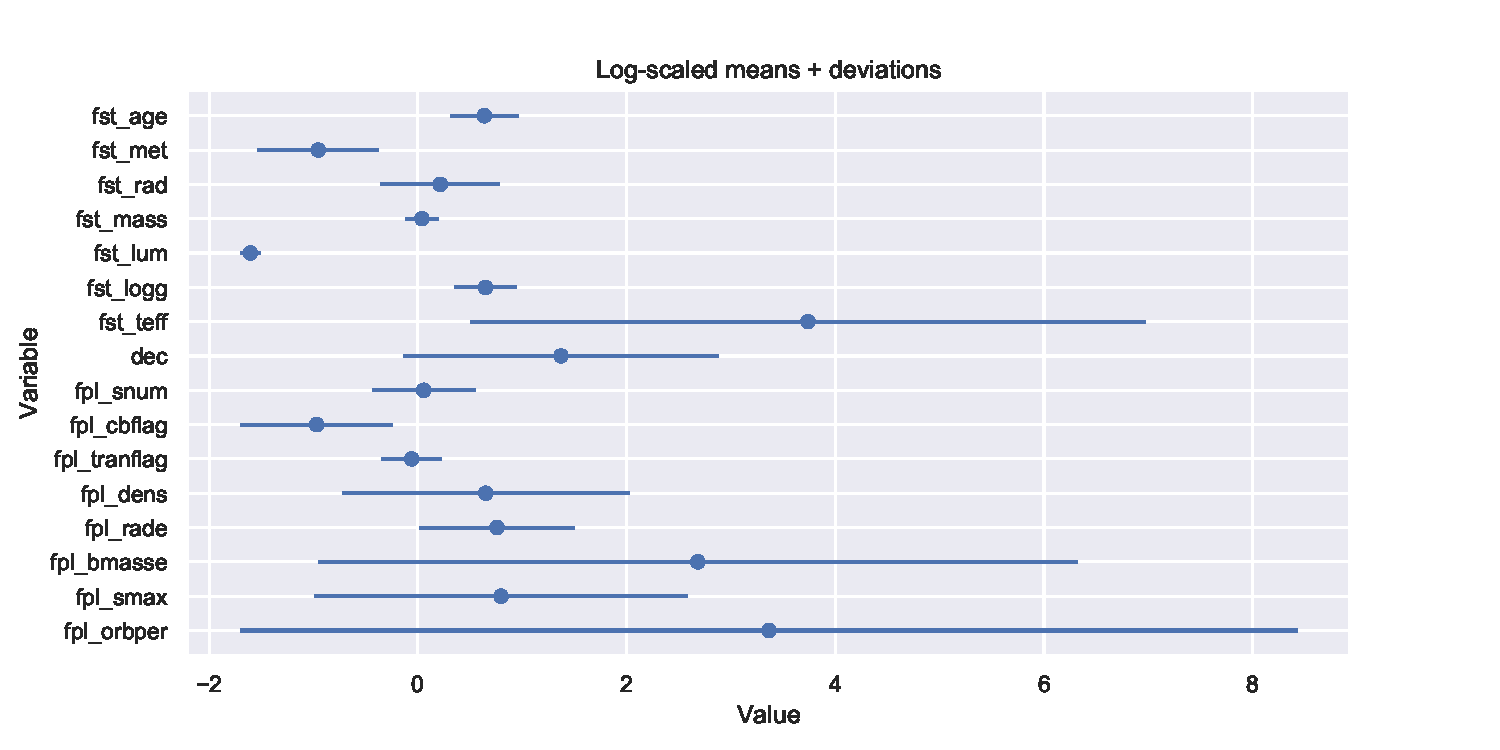
\includegraphics[angle=90, width=0.7\textwidth]{graphics/mean_deviation.pdf}
    \caption{log-scaled mean of each variable with its standard deviation}
    \label{pic:mean}
\end{figure}

\begin{figure}[!ht]\centering
    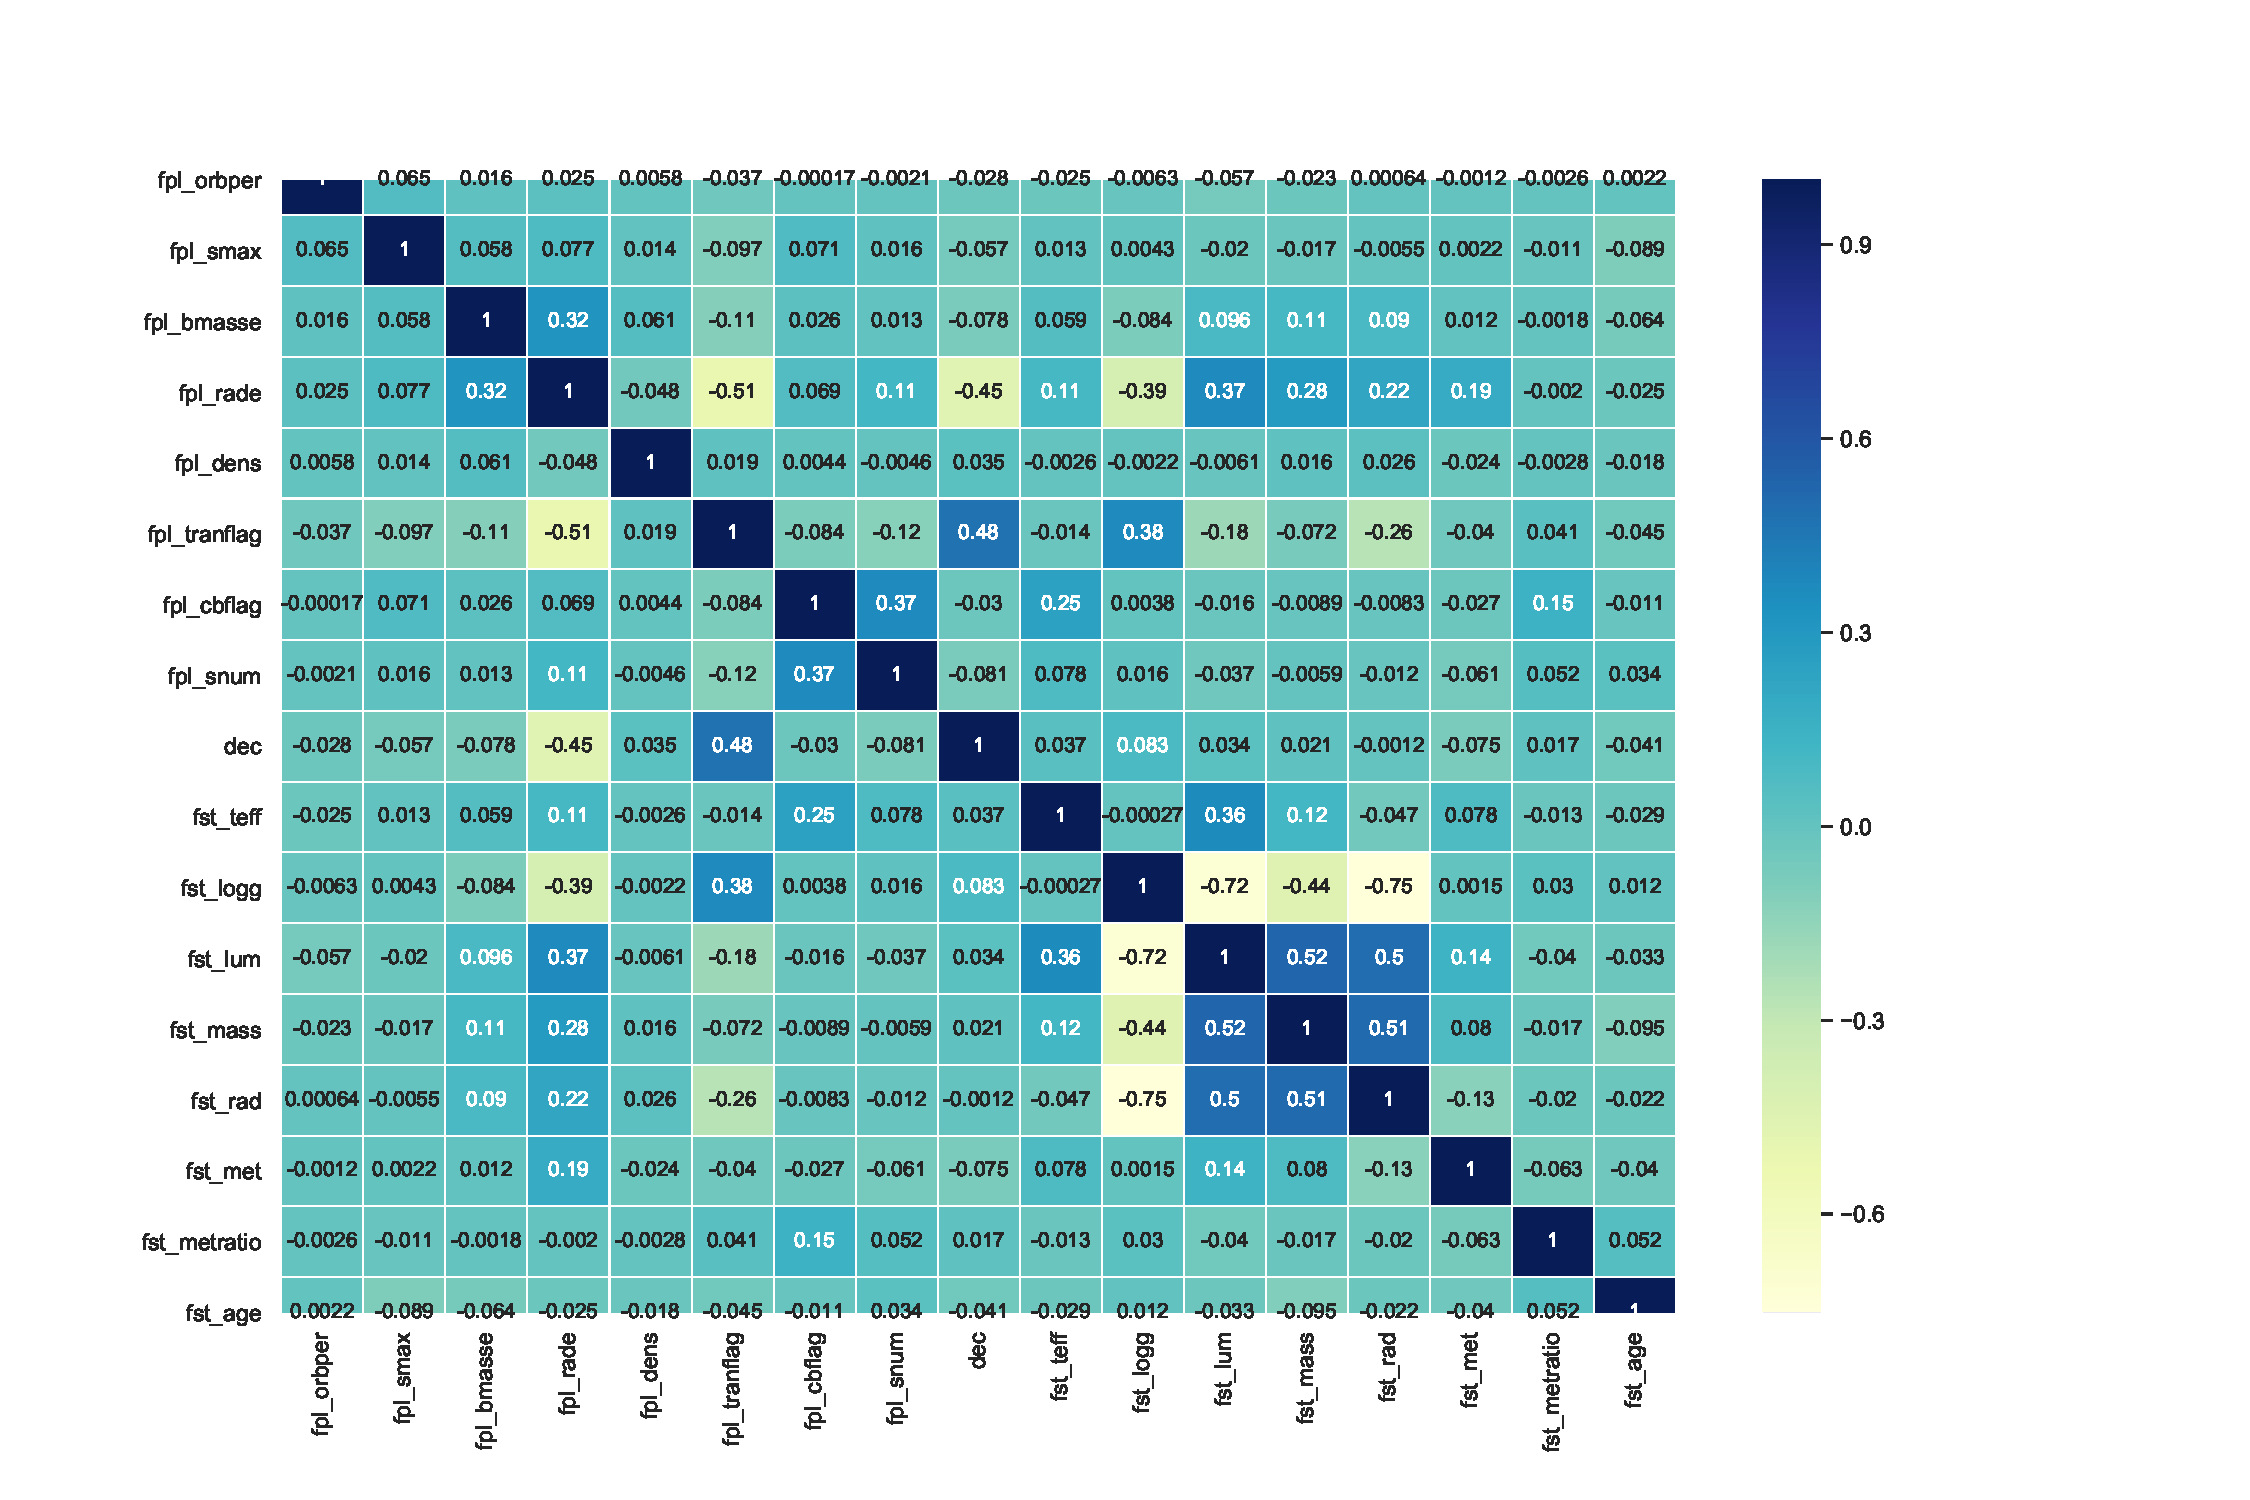
\includegraphics[angle=90, width=1\textwidth]{graphics/correlation_matrix.pdf}
    \caption{correlation matrix of variables}
    \label{pic:corr}
\end{figure}

\end{document}
